\documentclass[12pt]{article}
\usepackage[utf8]{inputenc}
\usepackage[T1]{fontenc}
\usepackage[english]{babel}
\usepackage{graphicx}
\usepackage{amsmath}
\usepackage{amssymb}
\usepackage{hyperref}
\usepackage{epsf}
\usepackage{float}
\usepackage{geometry}
\geometry{hmargin=3.5cm, vmargin=2.5cm}
\usepackage[squaren]{SIunits}
\usepackage{listings}
\usepackage{color}
\definecolor{mygreen}{RGB}{70, 180, 90}
\definecolor{mylilas}{RGB}{255, 117, 45}
\definecolor{cadr}{rgb}{0.89, 0.0, 0.13}
\graphicspath{{DWGs/}}
\usepackage{graphicx}
\usepackage{wrapfig}
\usepackage{graphicx}
\usepackage{multicol}
\usepackage{enumitem}
\usepackage{xcolor}
\usepackage{framed}
\definecolor{shadecolor}{RGB}{139, 231, 3}

\usepackage{tcolorbox}
\definecolor{mycolor}{rgb}{0.122, 0.435, 0.698}

\newtcbox{\mb}{nobeforeafter,colframe=mycolor,colback=mycolor!10!white,boxrule=0.5pt,arc=4pt,
  boxsep=0pt,left=6pt,right=6pt,top=3pt,bottom=3pt,tcbox raise base}


\begin{document}

\begin{titlepage}
    \begin{center}

		\vspace*{6cm}
        \LARGE     
		
        \Huge
        \textbf{Fluid Toolbox}
        
        \vspace*{1cm}
        


        \vspace{2cm}
        
        \LARGE
        K. Zdybal

        \vspace{6cm}
		\Large

		\vspace{1cm}

 		January, 2018 - $\infty$
	\end{center}
\end{titlepage}


% EX_LIBRIS_PAGE_TEMPLATE START ===============================

\thispagestyle{empty}
\begin{center}
    
\vspace*{4cm}

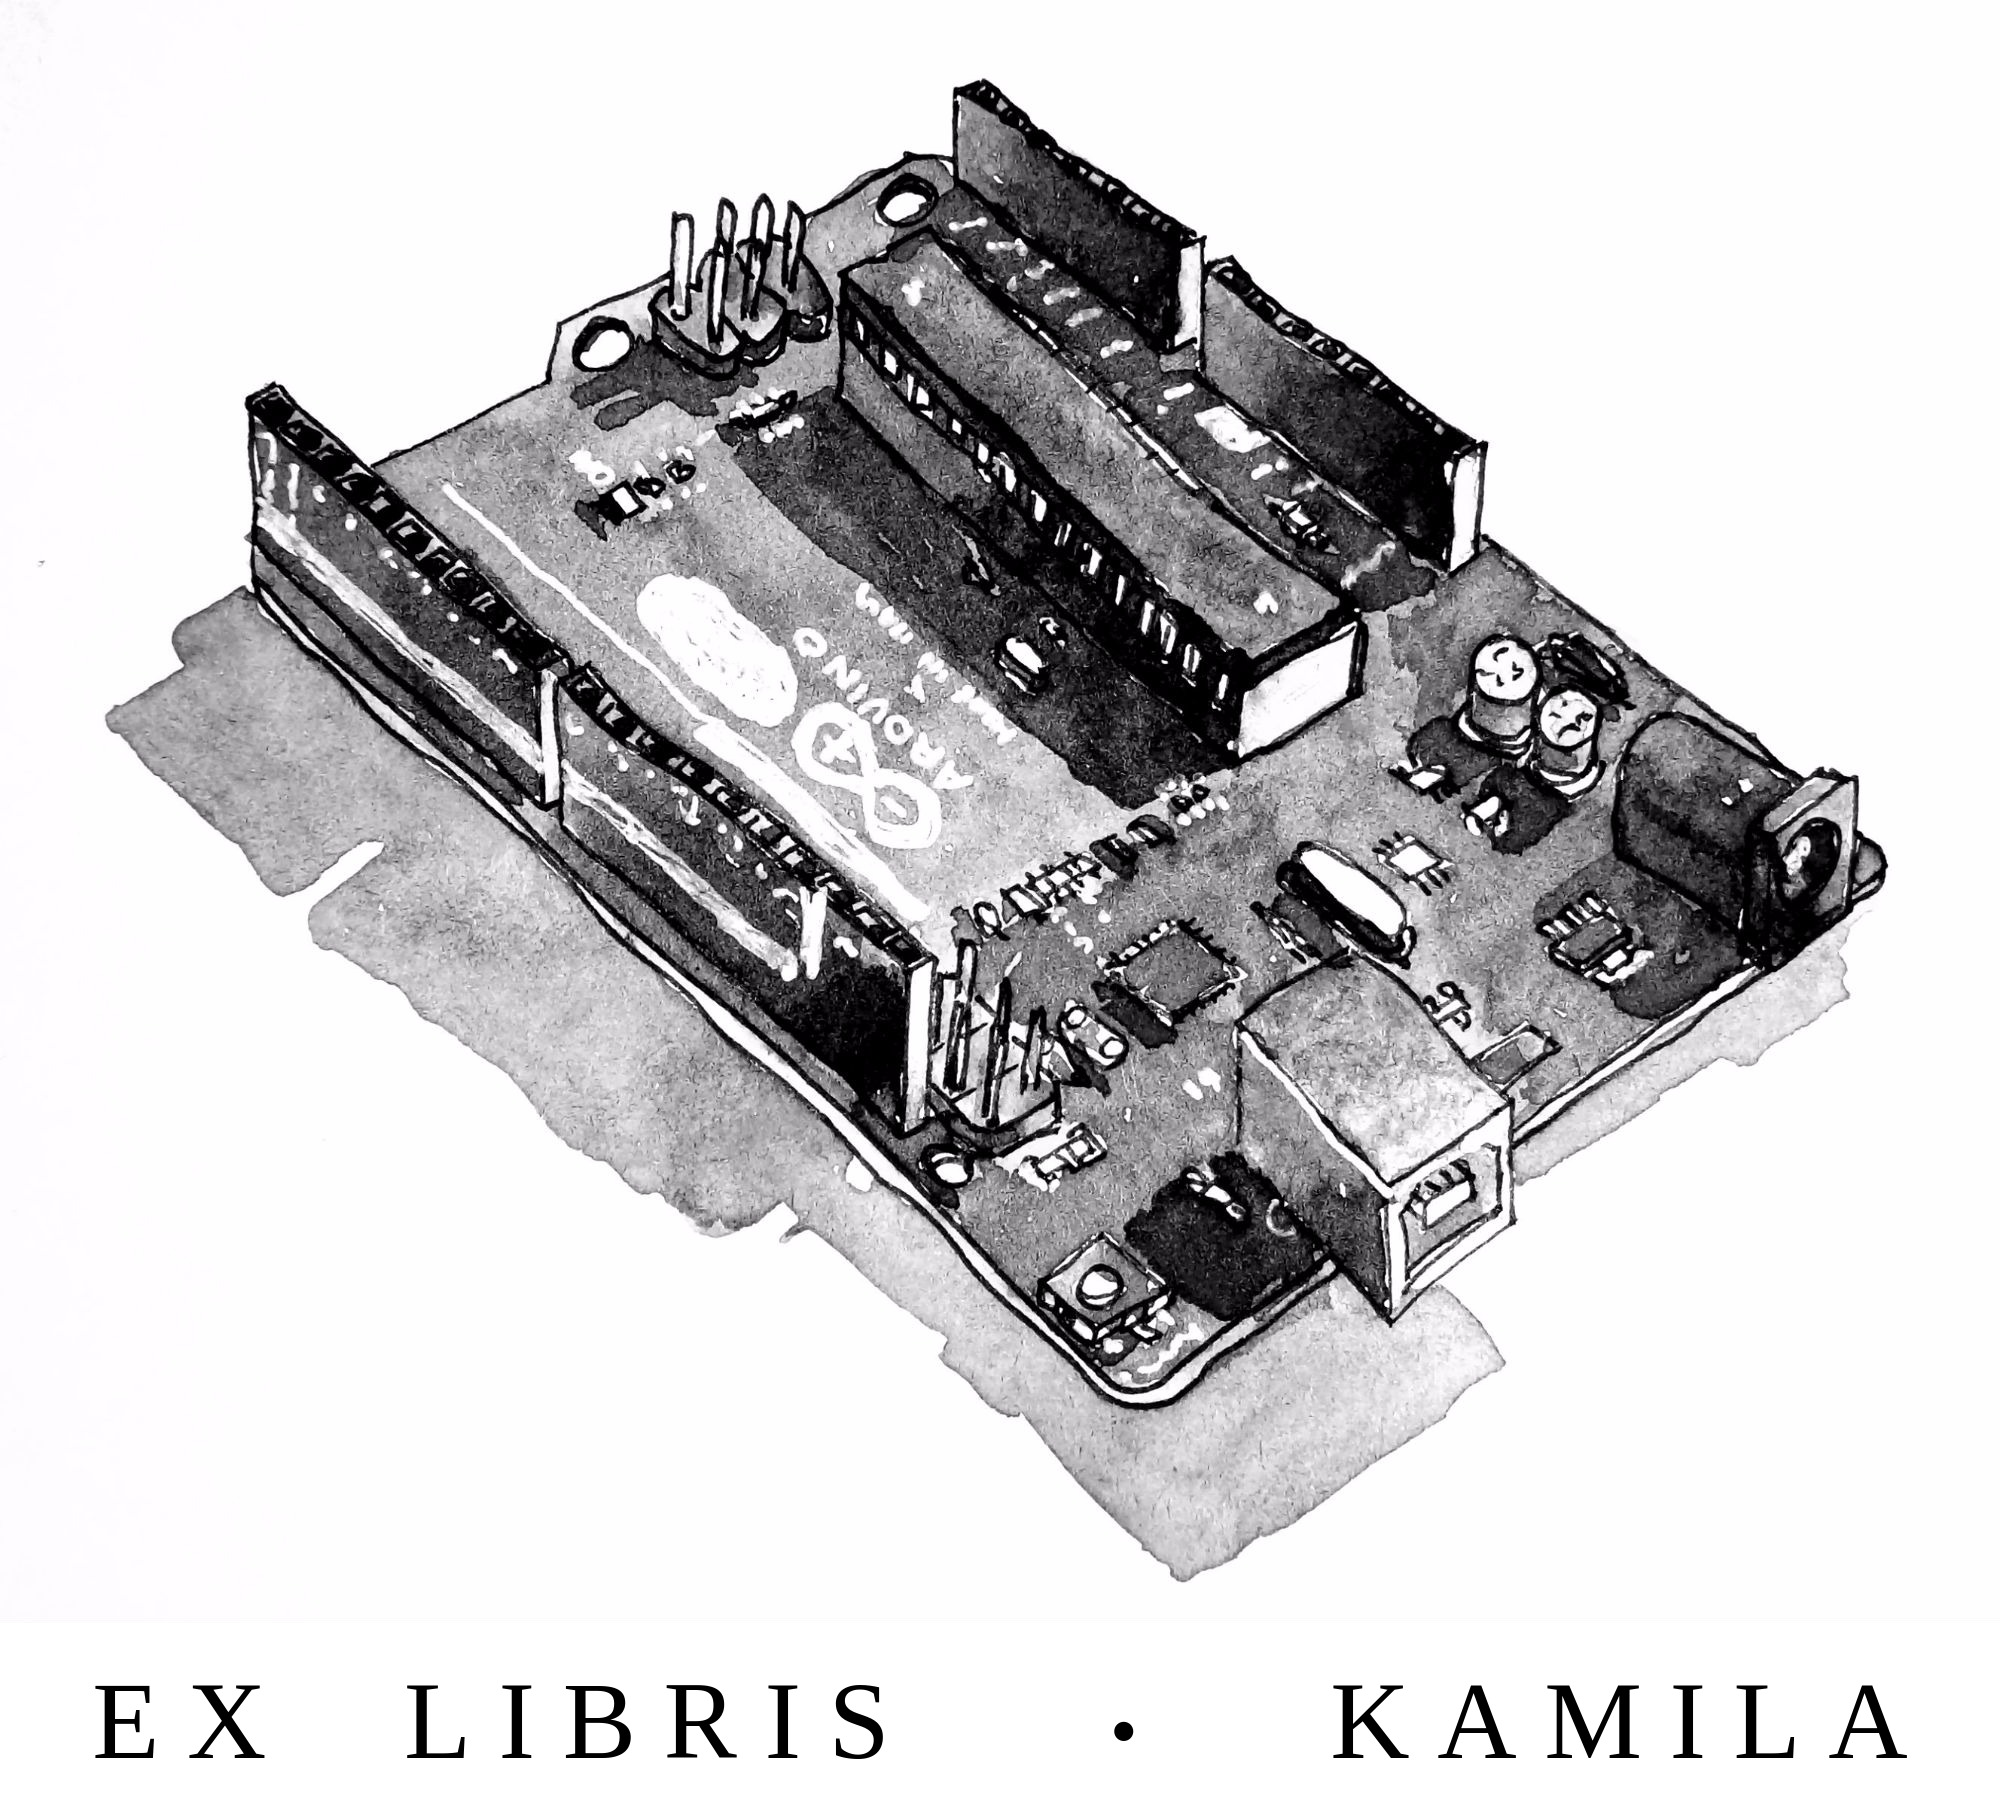
\includegraphics[width = 70mm]{arduino_dwg.jpg}

\vspace*{2cm}

Copyright \textcopyright \, Kamila Zdybał, 2018

For more documents similar to this one 

visit me on GitHub: @camillejr

To contact me personally drop me a line at:

\verb|kamilazdybal@gmail.com|

\end{center}
\newpage

% EX_LIBRIS_PAGE_TEMPLATE END ================================

\setlength{\parindent}{0cm}

\clearpage


\tableofcontents



\setlength{\parskip}{1em}
\renewcommand{\baselinestretch}{1.0}


\newpage


\section{Introduction} \label{chap:intro}



\section{Circulation}

\begin{equation}
\Gamma = \int \vec{\upsilon} \cdot \vec{dl}
\end{equation}

Questions:

\begin{enumerate}
\item Why closed loop? Would it have any meaning if we calculated circulation along any general spline?

\item How to chose the loops so that the circulation we calculate is of the most meaning to us?

\item What does the zero, positive, negative circulation mean?

\item Can circulation be infinite?

\end{enumerate}



\section{Vorticity}


\newpage

\begin{thebibliography}{50}



\end{thebibliography}

\end{document}
